\chapter{Integrals of motion}
\thispagestyle{chapterBeginStyle}

\paragraph{}The problem of our interest is the systematic classification of all local and quasilocal integrals of
motion (LIOMs and QLIOMs) supported on \(\NN \ni m \leq L/2\) sites. To this end, we employ the algorithm first proposed
in~\textcite{Mierzejewski2015a}, valid for any quantum lattice model. The aim of this thesis is to provide a pedagogical introduction to the topic, 
so all derivations are presented in full detail, together with a simple proof of correctness for the algorithm.

%%%%%%%%%%%%%%%%%%%%%%%%%%%%%%%%%%%%%%%%%%%%%%%%%%%%%%%%%%%%%%%%%%%%%%%%%%%%%%%%%%%%%%%%%%%%%%%%%%%%%%%%%%%%%%%%%%%%%%%%%%%%%%%%
\section{Preliminaries}

\paragraph{Locality} We begin with a definition of integral of motion in quantum mechanics.
\begin{definition}
  Let \(H\) be a Hamiltonian operator. Then, any observable \(O\) fulfilling the equation:
  \[
    \comm{H}{O} = 0
  \]
  is an \textbf{integral of motion}.\label{def:iom}
\end{definition}
It is easy to see, that there are many such observables. Let us consider the following
\begin{example}
  Take \(H\) to be any Hamiltonian operator. By spectral theorem, it can be written is diagonal form:
  \begin{equation*}
    H = \sum_n E_n \ketbra{n}{n}
  \end{equation*}
  Then a set of projection operators \(P_n = \ketbra{n}{n}\) is a family of IOMs.
  Eigenstates of a Hamiltonian are in general very nonlocal. \label{ex: projectors}
\end{example}
However, as it will become evident in Section~\ref{sec:spectral function} on spectral function, nonlocal operators are not important in the
thermodynamic limit and we are only interested in the so called local (or quasilocal) integrals of motion.
A working intuition behind local operators is perhaps best seen in Figure~\ref{fig:1D chain}. They can be thought of as
being different from identity only on \(m\) consecutive sites. XXZ Hamiltonian defined by equation~\eqref{eq:HXXZ} is an
example of 2-local operator.
\begin{figure}[!htbp]
  \centering
  \hspace*{-0.5cm}
  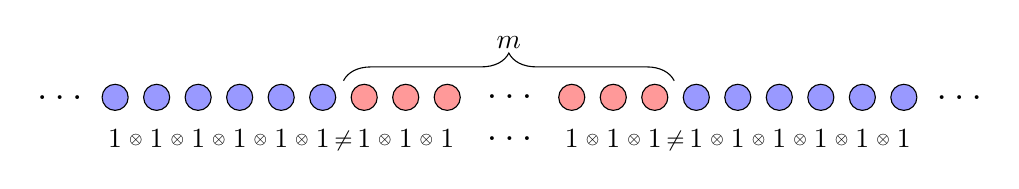
\begin{tikzpicture}[node distance = 15pt, auto]
    \tikzstyle{line} = [draw, -latex',thick]
    \tikzstyle{site1}=[circle, draw, fill=blue!40]
    \tikzstyle{site2}=[circle, draw, fill=red!40]
      % Place nodes

    \node [site1] (site-1) at (-8, 0) {};
    \foreach \x / \name in {1/2,2/3,3/4,4/5,5/6}      
      \node [site1, right of=site-\x] (site-\name) {};

    \node [site2, right of =site-6] (site-7){};
    \foreach \x / \name in {7/8,8/9}      
      \node [site2, right of=site-\x] (site-\name) {};

    \node [site2, right of=site-9, node distance=45pt] (site-10){};
    \foreach \x / \name in {10/11,11/12}      
      \node [site2, right of=site-\x] (site-\name) {};

    \node[site1, right of=site-12] (site-13){};
    \foreach \x / \name in {13/14,14/15,15/16,16/17,17/18}      
      \node [site1, right of=site-\x] (site-\name) {};

    \node [left of=site-1, node distance=20pt] {\Large $ \ldots $};
    \node [right of=site-18, node distance=20pt] {\Large $ \ldots $};
    
      
    \foreach \x in {1,...,18}     
      \node [black, below of=site-\x](op-\x) {\(\mathbb{1}\)};

    \foreach \x / \y in {1/2,2/3,3/4,4/5,5/6,7/8,8/9,10/11,11/12,13/14,14/15,15/16,16/17,17/18}
      \path[draw=none] (op-\x) -- (op-\y) node [black,midway,yshift=-6pt] {\tiny$\otimes$};
    
    \path[draw=none] (op-6) -- (op-7) node [black,midway,yshift=-8pt] {\footnotesize$\neq$};
    \path[draw=none] (op-12) -- (op-13) node [black,midway,yshift=-8pt] {\footnotesize$\neq$};
    % \foreach \x in {-1.5,-1.0,-0.5,0.5,1.0,1.5}
      % \node [site2] (site-\x) at (\x, 0) {};
      
      \draw [decorate,decoration={brace,amplitude=10pt},yshift=6pt] 
      (-5.1,0) -- (-0.9,0) node [black,midway,yshift=8pt] {$m$};
      
      \path [draw=none] (site-9) -- (site-10) node [black,midway,yshift=-4pt] {\Large$\ldots$};
      \path [draw=none] (op-9) -- (op-10) node [black,midway,yshift=-4pt] {\Large$\ldots$};
    \end{tikzpicture}
  \caption{Illustration of an operator supported on \(m\) sites.}
  \label{fig:1D chain}
\end{figure}
In Section~\ref{sec:algorithm}, a precise definition of locality and quasilocality will be stated.

\paragraph{Noncommutativity}In the case of XXZ model (also in general XYZ model) the Hamiltonian preserves the total \(z\)-component of spin,
or in other words, it commutes with the total spin operator of the form:
\begin{equation*}
  \Sz_{tot} = \sum_{i = 1}^{L} \Sz_i
\end{equation*} 
This fact allows us to decompose the full Hilbert space into parts consisting of states with the same total \(z\)-component
of spin. In more mathematical terms, we have the following:
\begin{equation*}
  \mathcal{H} = \bigoplus_{i = 0}^{L} \mathcal{H}_i \text{, where } \big(\forall \ket{\psi} \in \mathcal{H}_i \big) \big(\Sz_{tot} \ket{\psi} = \frac{1}{2}(i-L) \ket{\psi} \big)
\end{equation*}
i.e. the full Hilbert space with \(\dim{\mathcal{H}} = 2^L\) can be decomposed into the direct sum of its proper subspaces
\(\mathcal{H}_i\) such that \(\dim{\mathcal{H}_i} = \binom{L}{i}\) and all states in a given subspace correspond to the same
eigenvalue of \(\Sz_{tot}\) operator. The index \(i\) denotes the number of sites with spin up. 
Now we are ready for
\begin{definition}
  Let \(O\) be an integral of motion. If \(O\) preserves total \(z\)-component of spin, i.e.
  \(\comm{\Sz_{tot}}{O} = 0\), then it is called a \textbf{commuting integral of motion}.
  Otherwise, it is called a \textbf{noncommuting integral of motion}.\label{def:noncomm def}
\end{definition}
For the algorithm described in Section~\ref{sec:algorithm}, we need to construct matrices of
observables and express them in the Hamiltonian eigenbasis. If the operator in question is a
commuting IOM, we can restrict ourselves to the fixed spin subspace and thus greatly reduce
computational complexity, allowing us to investigate larger systems. Such operators, for example
spin energy current, have already been studied~\autocite{Mierzejewski2015Approx}. Therefore,
the main focus of this work is the investigation of existence and properties of much less known
noncommuting IOMs. This forces us to remain in full Hilbert space and restricts system sizes
that we are able to check.

%%%%%%%%%%%%%%%%%%%%%%%%%%%%%%%%%%%%%%%%%%%%%%%%%%%%%%%%%%%%%%%%%%%%%%%%%%%%%%%%%%%%%%%%%%%%%%%%%%%%%%%%%%%%%%%%%%%%%%%%%%%%%%%%

\section{(Q)LIOMs finding algorithm \label{sec:algorithm}}
  \paragraph{}Consider the vector space \(\mathcal{V}_L\) of traceless and translationally invariant
  observables, acting on a Hilbert space of dimension \(2^L\). We can define an inner product on this space:
  \begin{equation}
      \hs{A}{B} = \frac{1}{2^L}\tr(A^{\dagger}B) = \frac{1}{2^L} \sum_{mn} A_{nm}B_{nm}^{\ast}
  \end{equation}
  i.e. the Hilbert-Schmidt product, where \(A_{nm} = \matrixel{n}{A}{m}\) and \(H\ket{n} = E_n \ket{n}\). 
  This definition is correct, as we work only with finite dimensional Hilbert spaces and taking the trace is an
  linear operation. We require the operators to be traceless, because they have zero overlap with the identity, \(\left(A|\Id\right)=\frac{1}{2^L}\tr(A) = 0\).
  
  Now we introduce a subspace \(\mathcal{V}_L^m\) of \(m\)-local operators and a direct sum 
  \(\mathcal{V}_L^M = \bigoplus_{m = 1}^M \mathcal{V}_L^m\) being a subspace of operators supported on up to \(M\) sites.
  We also introduce a basis of \(\mathcal{V}_L^M\) consisting of operators \(O_s\in \mathcal{V}_L^M\)
  satisfying the following properties:
  \begin{align*}
    & \hs{O_s}{O_{t}} = \delta_{s,t} \tag{\text{orthonormality}}\\
    & \big(\forall A \in \mathcal{V}_L^M\big) \big(A = \sum_s \hs{O_s}{A} O_s\big) \tag{\text{completeness}}\\
    & \big(\forall A \in \mathcal{V}_L \big) \big( A = A^m + A^{\perp} = \sum_s \hs{O_s}{A} O_s + A^{\perp}\big) ,
     \text{ such that } \big(\forall s\big) \big( \hs{O_s}{A^{\perp}} = 0\big) 
  \end{align*}
  

  % Now we introduce an orthonormal basis of \({\mathcal{A}_L^m}\):
  % \begin{equation}
  %     O_{\underline{s} } = \sum_{j = 1}^L \sigma_{j}^{s_1}\sigma_{j+1}^{s_2}\cdots \sigma_{j+m-1}^{s_m}
  % \end{equation}
  % where \(\sigma^z_j \equiv \sqrt{2}S^{z}_j\), \(\sigma^{\pm}_j \equiv S^{\pm}_j\), \(\sigma^0_j\equiv \Id\), \(\underline{s} = (s_1,s_2,\ldots s_m)\)
  % and \(s_j \in \{+,-,z,0\}\) while \(s_{1,m} \in \{+,-,z\}\). For a fixed m, there are exactly \(N_m = 3\cdot 4^{m-2}\cdot 3\) such operators and they
  % satisfy an orthonormality condition i.e \(\left(O_{\underline{s}}|O_{\underline{s'}}\right) = \delta_{\underline{s},\underline{s'}}\). 
  
  % We define the infinite time averaging of an operator \(A\in \mathcal{A}_L^m\), employing the Heisenberg picture:
  % \begin{align}
  % \overline{A} = &\lim_{\tau \rightarrow \infty} \frac{1}{\tau} \int dt\, A_{H}(t) =  \nonumber
  % \lim_{\tau \rightarrow \infty} \frac{1}{\tau} \int dt\, e^{i H t}A e^{-i H t} = \\ \nonumber
  % &\sum_{n,m} \lim_{\tau \rightarrow \infty} \frac{1}{\tau} \int dt\, e^{i E_m t}\ket{m}  
  % \matrixel{m}{A}{n}\bra{n}  e^{-i E_n t} = \\ 
  % & \sum_{n,m} \matrixel{m}{A}{n}\ketbra{m}{n} \lim_{\tau \rightarrow \infty} \frac{1}{\tau}
  % \int dt \, e^{i(E_m-E_n)t} =  \sum_{n,m}^{E_n = E_m} \matrixel{m}{A}{n}\ketbra{m}{n}
  % \label{eq:time_avg}
  % \end{align}
  % It is evident from equation~\eqref{eq:time_avg} that large degeneracy of energy spectrum will be important to the
  % structure of time-averaged operators. Moreover, time averaging in such form is an orthogonal projection in the
  % Hilbert space of operators. From that follows a crucial property i.e \(\left(\overline{A}|\overline{B}\right) = 
  % \left(\overline{A}|B\right)\).
  
  \textcolor{blue}{Here continues a detailed derivation of the algorithm.}
  Operators with corresponding to largest eigenvalues of \(K\) matrix 
  
%%%%%%%%%%%%%%%%%%%%%%%%%%%%%%%%%%%%%%%%%%%%%%%%%%%%%%%%%%%%%%%%%%%%%%%%%%%%%%%%%%%%%%%%%%%%%%%%%%%%%%%%%%%%%%%%%%%%%%%%%%%%%%%%

  \section{Spectral function\label{sec:spectral function}}

  \paragraph{}One may ask a question, why are local (and quasilocal) IOMs actually important. To answer this
  question in a convincing manner we will follow the discussion in~\textcite{Vidmar2021} and
  introduce spectral functions. Suppose that we have an observable  

%%%%%%%%%%%%%%%%%%%%%%%%%%%%%%%%%%%%%%%%%%%%%%%%%%%%%%%%%%%%%%%%%%%%%%%%%%%%%%%%%%%%%%%%%%%%%%%%%%%%%%%%%%%%%%%%%%%%%%%%%%%%%%%%

\section{Commuting QLIOM: Spin energy current}

\paragraph{}In order to test our QLIOM finding algorithm and the correctness of its implementation, we investigate the known case of
energy current in Spin\(-1/2\) XXZ model~\autocite*{Mierzejewski2015Approx}. For the sake of completeness, derivation of
spin energy current for the general XYZ model will be presented, following the definitions in \textcite{Zotos1997}.
We start with the general XYZ Hamiltonian with periodic boundary conditions:
\begin{equation}
    H_{XYZ} = \sum_{i=1}^L  \left( J_{x} \Sx_{i}\Sx_{i+1} + J_{x} \Sy_{i}\Sy_{i+1} + J_{z} \Sz_{i}\Sz_{i+1} \right)
\end{equation}
It is easy to see that this Hamiltonian can be represented as a sum of operators supported on two consecutive sites:
\begin{equation}
    H_{XYZ} = \sum_{i=1}^L h_{i,i+1}
\end{equation}
where \(h_{i,i+1} = J_{x} \Sx_{i}\Sx_{i+1} + J_{x} \Sy_{i}\Sy_{i+1} + J_{z} \Sz_{i}\Sz_{i+1} \) and periodic boundary conditions
require that \(h_{L,L+1} = h_{L,1}\). The energy operator is a conserved quantity, thus the time evolution of its local density
is given by the discrete continuity equation:
\begin{equation}
    \dv{h_{i,i+1}(t)}{t} + \div{j_{i}^{E}(t)} = 0 
    \label{eq:discrete continuity}
\end{equation}
where \(\div{j_{i}^E(t)} \equiv j_{i+1}^E(t) - j_{i}^E(t)\) is the discrete divergence of spin energy current density and \(h_{i,i+1}(t) = e^{i H_{XYZ}t} h_{i,i+1} e^{-i H_{XYZ} t}\).
On the other hand, time evolution of an arbitrary operator is determined
by the Heisenberg equations:
\begin{equation}
    \dv{h_{i,i+1}(t)}{t} = i \comm{H_{XYZ}}{h_{i,i+1}(t)}
    \label{eq:heisenberg equation}
\end{equation}
Combining equations~\eqref{eq:discrete continuity} and~\eqref{eq:heisenberg equation} we obtain the defining equations for
the spin energy current density:
\begin{equation}
    j_{i+1}^E - j_{i}^E = - i \comm{H_{XYZ}}{h_{i,i+1}} = i \comm{h_{i,i+1}}{H_{XYZ}} = i \sum_{k=1}^L \comm{h_{i,i+1}}{h_{k,k+1}} 
    \label{eq:energy current defining equation}
\end{equation}
Similar equations can be written for any operator being a sum of local operators such as
the total spin operator or particle number operator in fermionic models. Detailed solution to the equation~\eqref{eq:energy current defining equation}
is shown in Appendix~\ref{app:spin energy current derivation}. For the XXZ model we get the following expression: 
\begin{align*}
  j_i^E &= i \Big( \underbrace{2J \Sm_{i-1}\Sz_i \Sp_{i+1} + J \Delta \Sz_{i-1}\Sp_i \Sm_{i+1} + J\Delta \Sp_{i-1}\Sm_i\Sz_{i+1}}_{O_i} \\
  &- \underbrace{\left(2J \Sp_{i-1}\Sz_i \Sm_{i+1} + J\Delta \Sz_{i-1}\Sm_i \Sp_{i+1} + J\Delta \Sm_{i-1}\Sp_{i} \Sz_{i+1} \right)}_{O_i^{\dagger}}\Big) \nonumber \\
  &= i\left(O_i - O_i^{\dagger}\right)
\end{align*}
Obtaining the energy current operator is now simply the matter of summing over all the lattice sites:
\begin{equation}
    J^E = \sum_{i=1}^L j_i^E
    \label{eq:energy current}
\end{equation}

\textcolor{blue}{Tutaj dalej o tym że komutuje z H, stała funkcja autokorelacji i jak zanika przy zaburzeniu. Ale dopiero po rozdziale o algorytmie żeby notacja była ustalona}